\documentclass[11pt,twocolumn]{article}
\usepackage{fullpage}
\usepackage{url}
\usepackage[margin=1.8in]{geometry}
\usepackage{graphicx}
\begin{document}
\author{Ran Bernstein \\
\texttt{ranb@cs.technion.ac.il} \\
Department of Computer Science, Technion I.I.T, Haifa, Israel}
\title{Laban movement recognition from markerless motion capture sensor}
\maketitle
\begin{quote}{``Man moves in order to satisfy a need.`` ---\textup{Rudolph Laban}}
\end{quote}
\begin{abstract}
\textbf{Laban Movement Analysis (LMA), developed in the dance community
over the past seventy years, is an effective method for observing, describing, notating, and interpreting human
movement to enhance communication and expression in everyday and professional life.
Many applications that use motion capture data might be significantly
leveraged if the Laban qualities will be recognized automatically.
This paper presents an automated recognition method of Laban qualities from
motion capture skeletal recordings and it is demonstrated on the output of
Microsoft's Kinect V2 sensor.}
\end{abstract} 
\section{Introduction}
\subsection{Laban movement analysis}
LMA is a formal language for motion description 
invented by Rudolf Laban \cite{Laban} in the middle of the 20th 
century. LMA describes, interprets and documents mental 
states from both conscious and unconscious human 
motion based on Laban�s theories of Body, Effort, Shape, 
and Space. LMA has been used in the fields of dancing, 
acting, athletics, physical therapy, and psychology and 
behavioral science. Laban exercises are based on the belief that by observing and analyzing 
movements, both conscious and unconscious, it is possible to recognize the objectives 
of the mover and to become aware of an inner attitude that precedes an action. Laban 
helps actors create momentary moods and long-standing personality characteristic 
through movement. LMA work investigates the Flow, Space, Time and Weight of all
movement and helps actors think specifically about why their character may move in a jerky, fast, light and 
direct manner verses a heavy, slow, indirect and uninterrupted manner: 
\begin{itemize}
\item 
Flow: Bound or Free 
\item
Space: Direct or Indirect 
\item
Time: Sudden or Sustained 
\item
Weight: Strong or Light 
\end{itemize}
\subsection{Laban qualities automated recognition}
Several attempts were made in order to recognize Laban qualities, most of them
were made for emotion recognition in the context of Human Robot Interaction (HRI).
Masuda et al. generated emotional body motion for a human 
form robot \cite{Masuda}. Rett et al. proposed a human motion recognition 
system using a Bayesian reasoning framework \cite{Rett}. Common in 
these studies, computational LMA offers some evidence that 
motion conveys emotional information, and this information 
allows such systems to estimate qualitative changes of motion.
Kim et al. performed first steps in this direction with the Kinect sensor, in 
this paper we extend such kind of work.
\subsection{Kinect sensor data}
This following figure shows the skeleton that is provided by the Kinect's
software development kit that were use in this paper.
\begin{figure}[ht!]
\centering
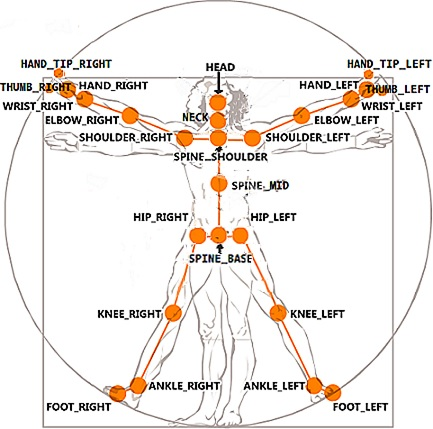
\includegraphics[width=60mm]{skeleton.jpg}
\caption{Skeleton positions relative to the human body}
\label{skeleton}
\end{figure}
Once the skeleton is detected, the 3D coordinates of all joints of user�s body 
� with the exception of joints, that are not visible (e.g. a user�s hand is
behind his back) are provided.
As seen in figure \ref{Coordinate}, the coordinates are in a �real-world�
coordinate system, that has the beginning [0,0,0] in the sensor, x,y and z-axis goes as shown on the picture below and the units are milimeters. 
\begin{figure}[ht!]
\centering
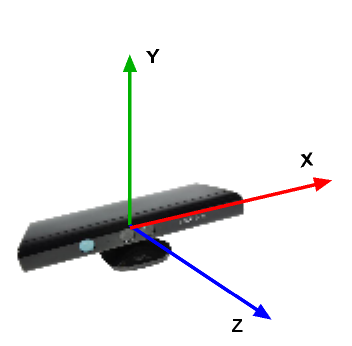
\includegraphics[width=60mm]{kinect_coordinate_system.png}
\caption{Kinect Coordinate System}
\label{Coordinate}
\end{figure}
\section{Method}
\subsection{Dataset collection}
The dataset was created by recording 5 Certified Movements Analysts (CMA)
performing random movements with several Laban qualities. Every clip is about
3 seconds long that were captured by the Kinect.
here goes table with an ellaboration about the amount of every quality every 

\subsection{Feature extraction}
Due to unequal length of clips, all the features that were extracted are in
whole clip granularity.
\subsubsection{Low level features}
For every joint in the skeleton the angular velocity, acceleration and jerk were
extracted, and for each one of them the mean, variance, skew and kurtosis were
extracted (the extraction of the last four moments is denoted as \phi). 
\subsubsection{Shape: Sagital}
In this quality a separation between Advance and Retreat. The quantification of
this quality was done by projecting the speed vector of the Center Of Mass (COM)
on the vector of the front of the body. The COM was approximated in this case
by the average of all of the joints. The front of the body was approximated by
the perpendicular vector to the the vector between the Left Shoulder (LS) and
the Right Shoulder (RS).
\\If $\vec{V}_{j}(t)$ is the vector of the position of joint j in time t in
clip with n frames, and $ \alpha_{j}$ is a coefficient proportional to the mass
around of the joint:
\\
\\\vec{V}_{COM}(t) = \sum_{j \in Joints} \alpha_{j}\vec{V}_{j}(t)
\\
\\\vec{V}_{shoulders}(t)=\vec{V}_{LS}(t)-\vec{V}_{RS}(t)
\\
\\\vec{V}_{front}=\vec{V}_{shoulders}\[ \left( \begin{array}{ccc}
0 & 0 & 1 \\
0 & 1 & 0 \\
-1 & 0 & 0 \end{array} \right)\] 
\\
\\S_{sag}(t) = \vec{V}_{COM}(t)\cdot\vec{V}_{front}(t)
\\
\\
\vec{F}_{sag} = \phi([S_{sag}(1), \ldots S_{sag}(n)])
\\
\\
Where $ \phi$ is the moments extraction.
\subsubsection{Shape: Horizontal}
Here the separation is between spreadind and enclosing in the horizontal axe.
This quality was quantified by measuring the average distance of the joint from
the the vertical axe of the body that spreads from the head along the spine.
\subsubsection{Effort}
\subsubsection{Time}
\subsection{Multi-label classification}
Multi-label learning deals with the problem where each instance is associated
with multiple labels simultaneously, where the number of labels is not fixed
between instance to instance. The task of this learning paradigm is to predict
the label (Laban quality) set for each unseen instance (skeletal recording), 
through analyzing training instances with known label sets. A one hidden layer 
neural network architecture was used, trained with backpropagation algorithm
with regularization. The evaluation was done using Hamming loss (the
percentage of the wrong labels to the total number of labels).
\section{Results}
\begin{thebibliography}{1}
\bibliographystyle{plain}
  \bibitem{Laban} Laban, Rudolf, and Lisa Ullmann. "The mastery of movement."
  (1971).
  \bibitem{Rett}J. Rett and J. Dias, �Bayesian reasoning for Laban Movement
  Analysis used in human-machine interaction,� International Journal of Reasoning-based 
  Intelligent Systems, Vol. 2, No. 1,pp. 13-35, 2010
  \bibitem{Masuda}M. Masuda and S. Kato, �Motion Rendering System for 
	Emotion Expression of Human Form Robots Based on Laban 
	Movement Anlaysis,� 19th IEEE International Symposium on 
	Robot and Human Interactive Communication, Italy, 2010. 
  \bibitem{Kim}Kim, Woo Hyun, et al. "LMA based emotional motion representation
  using RGB-D camera." Proceedings of the 8th ACM/IEEE international conference on Human-robot 
  interaction. IEEE Press, 2013.
   
 \end{thebibliography}
\end{document}
